Der Versuchsaufbau sieht wie in Abb. \eqref{Mess} dargestellt aus.
	\begin{figure}[h]
		\begin{center}
		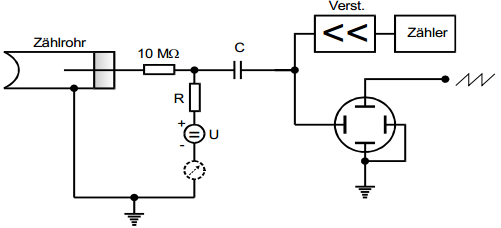
\includegraphics[scale=1.0]{Messaparatur.png}
		\caption{Skizze der Messaparatur [1]}
		\label{Mess}
		\end{center}	
	\end{figure}
\subsection{Charakteristik des Zählrohres}
Zur Aufnahme der Charakteristik des Zählrohres wird eine $\beta$-Quelle vor das Zählrohrfenster in festem Abstand gestellt.
Nun wird bis zum Erreichen des Plateaus in 3-$V$-Schritten die Zählrate gemessen, anschließend in 50 $V$-Schritten bis 650 $V$ und anschließend wieder in 3 $V$-Schritten bis etwa 700 $V$.
\subsection{Sichtbarmachung von Nachentladungen}
In diesem qualitativen Experiment wird die Strahlungsintensität soweit abgesenkt, dass auf dem Oszilloskop praktisch kein weiterer Impuls eines weiteren $\beta$-Teilchens zu sehen ist. Hier liegt die Zählrohrspannung bei etwa 350 $V$. Anschließend wird die Zählrohrspannung auf etwa 700 $V$ erhöht.
Nun lässt sich grafisch am Oszilloskop die Zeit zwischen Primär- und Nachentladungsimpuls ablesen.
\subsection{Messung Totzeit}
Bei hoher Strahlungsintensität wird das Oszilloskop so eingestellt, dass sich etwa ein Bild wie in Abb. \eqref{Tot} einstellt. Nun lässt sich die Totzeit graphisch ablesen.\\
Die 2. Methode ist die 2-Quellenmethode. Hierbei wird zunächst die Zählrate der 1. Quelle bestimmt,anschließend die Zählrate beider Quellen zusammen und zuletzt die der 2. Quelle allein.Dann lässt sich die Totzeit nach folgender Formel berechnen:\\
\begin{align}
T=\frac{N_{1}+N_{2}-N_{1+2}}{2N_{1}N_{2}}
\label{2}
\end{align}\\
\subsection{ Messung pro Teilchen freigesetzte Ladung}
Mit einem Strommessgerät wird bei der Aufnahme der Charakteristik des Zählrohres auch jeweils der Zählrohrstrom gemessen.
Die  freigesetzte Ladungsmenge lässt sich berechnen nach:\\
\begin{align}
\Delta Q=\frac{I \Delta t}{Z}
\label{ladungsmenge}
\end{align}\\
$\Delta$ Q hängt von $U$, wird also in Abhängigkeit davon untersucht.